\documentclass[11pt,a4paper]{article}
\usepackage{fontspec}
\setlength{\emergencystretch}{1em}
\usepackage[a4paper,top=18mm,bottom=20mm,left=19mm,right=19mm]{geometry}
\usepackage{booktabs,tabularx,array,multirow}
\usepackage{xcolor,tcolorbox}
\usepackage{amsmath,amssymb}
\usepackage{graphicx}
\usepackage{float}
\usepackage{pgfplots}
\usepackage{fancyhdr}
\usepackage{hyperref}
\usepackage{enumitem}
\usepackage{microtype}
\pgfplotsset{compat=1.18}

\definecolor{navy}{HTML}{17324D}
\definecolor{blue}{HTML}{2F6BFF}
\definecolor{teal}{HTML}{00A6A6}
\definecolor{orange}{HTML}{E9852D}
\definecolor{purple}{HTML}{7456B8}
\definecolor{rose}{HTML}{D45576}
\definecolor{green}{HTML}{3B9A66}
\definecolor{ink}{HTML}{263442}
\definecolor{muted}{HTML}{66788A}
\definecolor{panel}{HTML}{F3F6FA}
\definecolor{rule}{HTML}{D8E0E8}

\hypersetup{colorlinks=true,linkcolor=navy,urlcolor=blue,pdftitle={Sync2Act Mixed Modality Damage Study}}
\setlength{\parindent}{2em}
\setlength{\parskip}{0.25em}
\setlength{\headheight}{24pt}
\setlist{nosep,leftmargin=2em}
\renewcommand{\arraystretch}{1.22}
\pagestyle{fancy}
\fancyhf{}
\lhead{\textcolor{muted}{Sync2Act / Quality-Aware ACT}}
\rhead{\textcolor{muted}{Mixed-Modality Study}}
\cfoot{\textcolor{muted}{\thepage}}
\renewcommand{\headrulewidth}{0.4pt}
\renewcommand{\headrule}{\hbox to\headwidth{\color{rule}\leaders\hrule height \headrulewidth\hfill}}

\newcolumntype{Y}{>{\raggedright\arraybackslash}X}
\newcolumntype{C}[1]{>{\centering\arraybackslash}p{#1}}
\newcommand{\code}[1]{\texttt{\small #1}}
\newcommand{\good}[1]{\textcolor{green}{\bfseries #1}}
\newcommand{\warn}[1]{\textcolor{orange}{\bfseries #1}}

\begin{document}

\begin{titlepage}
\pagecolor{panel}
\vspace*{5mm}
{\color{blue}\rule{25mm}{2.5pt}}\\[7mm]
{\fontsize{22}{28}\selectfont\bfseries\color{navy} Sync2Act\\[2mm]
Mixed-Modality Data Corruption Study\par}
\vspace{5mm}
{\Large\color{muted}Full datasets, six ablations, three random seeds\par}
\vspace{8mm}

\begin{tcolorbox}[colback=white,colframe=rule,boxrule=0.7pt,arc=2mm,left=5mm,right=5mm,top=4mm,bottom=4mm]
\begin{tabularx}{\linewidth}{>{\bfseries\color{navy}}p{33mm}Y}
Experiment size & 3 datasets $\times$ 6 ablations $\times$ 5 conditions $\times$ 3 seeds\\
Completion & \good{270 / 270 runs completed and passed integrity audits}\\
Training scope & Full episodes, all frames and cameras; training-only corruption\\
Main metrics & Clean-test action MSE and ratios to the same model/seed's clean-training baseline\\
Ensembling & Existing checkpoints reused for paired causal-ensemble and first-step evaluation\\
Updated & Original study: 2026-09-25; supplementary evaluation: 2026-10-01
\end{tabularx}
\end{tcolorbox}

\vfill
{\large\color{ink}\bfseries Findings at a glance}\par
\vspace{2mm}
{\color{ink}For shifted or missing action labels, correctly aligned Oracle label quality nearly removes average degradation: Quality-Full has relative MSE $0.977\times$, versus ACT-Lite's $2.432\times$. Under mixed damage, the respective ratios are $1.144\times$ and $1.535\times$. State-quality input also helps, while image quality has no clear benefit under the current offline metric.\par}
\vspace{2mm}
{\small\color{ink}\textbf{Temporal-ensemble supplement: }A matching overall-results curve and actual before/after MSE comparisons have been added. Relative degradation and actual error changes are interpreted separately.\par}
\vspace{6mm}
{\small\color{muted}Experiment output: \code{runs/mixed\_modality\_damage\_v1\_3\_0} \hfill Sync2Act}
\end{titlepage}
\nopagecolor

\section{Research question and evidence boundaries}

This study examines four mixed-quality training conditions: image damage, state damage, action-label damage, and a mixture across modalities. When clean and damaged segments coexist, should modality-specific quality enter the model input, weight the loss, or do both?

Quality is \textbf{Oracle quality} supplied by the known synthetic corruption process. It encodes known fault provenance using heuristic scores, not calibrated correctness probabilities, a proven performance upper bound, or automatically available deployment signals. All results measure \textbf{offline action prediction} on clean test data. MSE and MAE do not substitute for closed-loop success, return, or safety-failure rates in simulation or hardware.

Original ablation results use the first action of each predicted chunk. Section 6 adds the same overall plot using temporal ensembling, plus separate actual MSE and percentage-change tables. The new plot divides by ensembled clean-training results; before/after tables compare against first-step evaluation. These denominators answer different questions.

\section{Datasets and training protocol}

The three robot datasets passed the single-task check. Training uses all recorded camera views in each dataset. A fixed episode-level split precedes training-only corruption, avoiding adjacent-frame leakage between training and testing.

\begin{table}[htbp]
\centering
\small
\begin{tabularx}{\linewidth}{Y C{14mm} C{18mm} C{14mm} C{22mm} C{24mm}}
\toprule
Dataset & Episode & Frame & Cameras & State / Action & Train / Val / Test\\
\midrule
XArm Lift Medium & 800 & 20,000 & 1 & 4 / 4 & 640 / 80 / 80\\
Koch Pick Place 1 Lego & 100 & 32,951 & 2 & 6 / 6 & 80 / 10 / 10\\
ALOHA Static Battery & 49 & 29,400 & 4 & 14 / 14 & 41 / 4 / 4\\
\bottomrule
\end{tabularx}
\caption{Full-dataset statistics. Training uses one, two, and four recorded camera views, respectively.}
\end{table}

Shared settings: 10 epochs, CUDA, batch size 256, segment length 16, training seeds 7/17/27, and split seed 7. The image longest edge is resized to 64 pixels. Normalization statistics are computed only from clean training episodes and frozen across all 90 combinations within a dataset. Validation and test remain clean.

\begin{tcolorbox}[colback=panel,colframe=rule,title={\color{navy}\bfseries Data separation and audits},fonttitle=\bfseries]
All 270 runs retain individual checkpoints, prediction CSVs, per-episode metrics, and manifests. Audits confirm matching checkpoint/quality schemas, experiment signatures, and run metadata; one normalization definition per dataset; and no missing or duplicate combinations.
\end{tcolorbox}

\clearpage\section{Mixed-corruption conditions}

Each episode is divided into contiguous segments, each assigned exclusively to one component according to mixture weights. A segment is not counted in multiple percentage buckets. Shifts use two frames with invalid boundaries marked missing. Modality missingness sets the corresponding input/label and quality to zero, and records missing masks and provenance.

\begin{table}[htbp]
\centering
\small
\begin{tabularx}{\linewidth}{p{39mm}Y}
\toprule
Training condition & Segment composition\\
\midrule
Clean & 100\% clean\\
Mixed image damaged & 50\% clean + 40\% image shift 2 + 10\% image missing\\
Mixed state damaged & 50\% clean + 40\% state shift 2 + 10\% state missing\\
Mixed action damaged & 50\% clean + 40\% action shift 2 + 10\% action-label missing\\
Mixed three corruptions & 20\% clean + 20\% image shift 2 + 20\% state shift 2 + 25\% action shift 2 + image/state/action missing, each 5\%\\
\bottomrule
\end{tabularx}
\caption{The five formal training conditions.}
\end{table}

Across datasets and seeds, segment proportions differ from targets by at most approximately 0.03 percentage points. Final episode segments can have fewer than 16 frames, so frame proportions differ slightly: by at most about 0.35 percentage points for single-modality conditions and 0.83 for the mixed condition.

\section{Six ACT / quality ablations}

\begin{table}[htbp]
\centering
\small
\begin{tabularx}{\linewidth}{p{38mm} C{24mm} C{26mm} Y}
\toprule
Model & Quality input & Label-weighted loss & Purpose\\
\midrule
ACT-Lite & No & No & Baseline without quality\\
Quality-Input & Yes & No & Input conditioning only\\
Quality-Weighted-Loss & No & Yes & Label downweighting only\\
Quality-Full & Yes & Yes & Full method\\
Quality-Shuffled & Shuffled & Yes & Break sample correspondence\\
Quality-Constant & Constant & Yes & Mark every sample as clean\\
\bottomrule
\end{tabularx}
\end{table}

Image/state missingness does not remove whole samples. Samples remain in training, and observation quality/missing masks describe unreliable inputs. Missing actions concern label reliability: only label-quality-weighted loss reduces or removes their supervision contribution.

\section{Metrics and aggregation}

The primary metric is action mean squared error on the clean test set:
\[
\mathrm{MSE}=\frac{1}{N d}\sum_{i=1}^{N}\lVert\hat{a}_i-a_i\rVert_2^2.
\]
Action units and scales differ across datasets. Cross-dataset aggregation therefore uses ratios within the same model and seed:
\[
R=\frac{\mathrm{MSE}_{\mathrm{damaged\ train}\rightarrow\mathrm{clean\ test}}}
{\mathrm{MSE}_{\mathrm{clean\ train}\rightarrow\mathrm{clean\ test}}}.
\]
$R=1$ matches clean training; $R>1$ indicates degradation. Overall results first compute $R$ within each dataset/model/seed, then average nine ratios across three datasets and three seeds.

\clearpage\section{Overall results}

\begin{figure}[H]
\centering
\begin{tikzpicture}
\begin{axis}[
width=0.99\linewidth,height=77mm,
ymin=0.85,ymax=2.65,
ylabel={Mean MSE ratio $R$},
symbolic x coords={Image,State,Action,Mixed},
xtick=data,
legend style={at={(0.5,-0.24)},anchor=north,legend columns=3,font=\scriptsize,draw=none},
grid=major,grid style={rule!60},axis line style={rule},tick style={rule},
every axis plot/.append style={thick,mark size=2pt}]
\addplot[color=navy,mark=*] coordinates {(Image,0.999)(State,1.388)(Action,2.432)(Mixed,1.535)};
\addlegendentry{ACT-Lite}
\addplot[color=blue,mark=square*] coordinates {(Image,0.995)(State,1.234)(Action,2.394)(Mixed,2.007)};
\addlegendentry{Quality-Input}
\addplot[color=orange,mark=triangle*] coordinates {(Image,1.000)(State,1.374)(Action,0.992)(Mixed,1.163)};
\addlegendentry{Weighted-Loss}
\addplot[color=teal,mark=diamond*] coordinates {(Image,0.996)(State,1.238)(Action,0.977)(Mixed,1.144)};
\addlegendentry{Quality-Full}
\addplot[color=rose,mark=pentagon*] coordinates {(Image,1.004)(State,1.449)(Action,2.463)(Mixed,1.538)};
\addlegendentry{Shuffled}
\addplot[color=purple,mark=x] coordinates {(Image,0.994)(State,1.303)(Action,2.401)(Mixed,1.500)};
\addlegendentry{Constant}
\addplot[color=muted,dashed,no marks] coordinates {(Image,1)(Mixed,1)};
\end{axis}
\end{tikzpicture}
\caption{Mean relative MSE across three datasets and three seeds. Lower is better; the dashed line denotes clean training.}
\end{figure}

\begin{table}[H]
\centering
\small
\begin{tabular}{lrrrr}
\toprule
Model & Image damaged & State damaged & Action damaged & Mixed\\
\midrule
ACT-Lite & 0.999 & 1.388 & 2.432 & 1.535\\
Quality-Input & 0.995 & \good{1.234} & 2.394 & 2.007\\
Weighted-Loss & 1.000 & 1.374 & 0.992 & 1.163\\
Quality-Full & 0.996 & 1.238 & \good{0.977} & \good{1.144}\\
Shuffled & 1.004 & 1.449 & 2.463 & 1.538\\
Constant & \good{0.994} & 1.303 & 2.401 & 1.500\\
\bottomrule
\end{tabular}
\caption{Mean MSE ratios. Green marks column minima, not statistical significance.}
\end{table}

% temporal-ensemble:start
\clearpage\subsection{Overall results with temporal ensembling}
Reuse 270 checkpoints and the original test episodes, without retraining; decay=0.7 was fixed before evaluation. Only predictions from chunks starting at or before the target time are fused; history resets at episode boundaries. Historical first-step prediction audits passed: 270/270 passed.
Normalization matches the original Section 6 plot: within each dataset/model/seed, divide the condition's test MSE by that model and seed's clean-training test MSE, then average nine ratios. Both numerator and denominator use ensembled MSE. Categories, six-model colors, and the vertical range match the original plot.
\[R_{\mathrm{ens}}=\frac{\mathrm{MSE}_{\mathrm{damaged\ train,\ ens}}}{\mathrm{MSE}_{\mathrm{clean\ train,\ ens}}}.\]
\begin{figure}[H]\centering\begin{tikzpicture}\begin{axis}[
width=0.99\linewidth,height=77mm,ymin=0.85,ymax=2.65,ylabel={Mean MSE ratio $R_{\mathrm{ens}}$},
symbolic x coords={Image,State,Action,Mixed},xtick=data,
legend style={at={(0.5,-0.24)},anchor=north,legend columns=3,font=\scriptsize,draw=none},
grid=major,grid style={rule!60},axis line style={rule},tick style={rule},every axis plot/.append style={thick,mark size=2pt}]
\addplot[color=navy,mark=*] coordinates {(Image,1.00116827)(State,1.25143456)(Action,2.11772046)(Mixed,1.40696803)};
\addlegendentry{ACT-Lite}
\addplot[color=blue,mark=square*] coordinates {(Image,1.00154140)(State,1.13276081)(Action,2.07105085)(Mixed,1.68312694)};
\addlegendentry{Quality-Input}
\addplot[color=orange,mark=triangle*] coordinates {(Image,1.00175641)(State,1.24646481)(Action,1.00888235)(Mixed,1.12149579)};
\addlegendentry{Weighted-Loss}
\addplot[color=teal,mark=diamond*] coordinates {(Image,1.00215427)(State,1.13595354)(Action,1.00021420)(Mixed,1.09702286)};
\addlegendentry{Quality-Full}
\addplot[color=rose,mark=pentagon*] coordinates {(Image,1.00914090)(State,1.26358199)(Action,2.10738241)(Mixed,1.37870756)};
\addlegendentry{Shuffled}
\addplot[color=purple,mark=x] coordinates {(Image,0.99985525)(State,1.19589319)(Action,2.07474105)(Mixed,1.39162016)};
\addlegendentry{Constant}
\addplot[color=muted,dashed,no marks] coordinates {(Image,1)(Mixed,1)};
\end{axis}\end{tikzpicture}\caption{Mean relative MSE with temporal ensembling. Each point averages nine ratios (three datasets, three seeds); the dashed line is the ensembled clean-training baseline.}\end{figure}
\begin{table}[H]\centering\small\begin{tabular}{lrrrr}\toprule
Model & Image & State & Action & Mixed\\\midrule
ACT-Lite & 1.0012 & 1.2514 & 2.1177 & 1.4070\\
Quality-Input & 1.0015 & 1.1328 & 2.0711 & 1.6831\\
Weighted-Loss & 1.0018 & 1.2465 & 1.0089 & 1.1215\\
Quality-Full & 1.0022 & 1.1360 & 1.0002 & 1.0970\\
Shuffled & 1.0091 & 1.2636 & 2.1074 & 1.3787\\
Constant & 0.9999 & 1.1959 & 2.0747 & 1.3916\\
\bottomrule\end{tabular}\caption{Values from the new plot: degradation relative to clean training, not ensemble-versus-first-step changes.}\end{table}
\clearpage\subsection{MSE before and after ensembling}
\begingroup\small\renewcommand{\arraystretch}{1.08}\setlength{\intextsep}{8pt}
Compute 100 times (ensemble MSE / first-step MSE - 1) per run, then average over three datasets and three seeds. Negative values mean lower MSE; positive values mean higher MSE. Raw MSE is not averaged across robots.
\begin{table}[H]\centering\small\begin{tabularx}{\linewidth}{Yrrrrr}\toprule
Model & Clean & Image & State & Action & Mixed\\\midrule
ACT-Lite & +27.37\% & +27.72\% & +15.23\% & +11.47\% & +16.74\%\\
Quality-Input & +27.65\% & +28.58\% & +17.27\% & +11.29\% & +8.59\%\\
Weighted-Loss & +27.32\% & +27.68\% & +15.87\% & +29.56\% & +22.52\%\\
Quality-Full & +27.67\% & +28.46\% & +17.22\% & +31.16\% & +22.64\%\\
Shuffled & +27.51\% & +28.10\% & +11.55\% & +10.29\% & +14.60\%\\
Constant & +27.58\% & +28.29\% & +17.16\% & +11.10\% & +17.89\%\\
\bottomrule\end{tabularx}\caption{Mean paired MSE changes. Each cell averages nine runs; positive values mean increased error.}\end{table}
Each row below averages 15 runs within one dataset/model: five training conditions and three seeds. MSE difference = ensemble mean - first-step mean; change (\%) = 100 times (ensemble mean / first-step mean - 1). This ratio of means differs from the mean of per-run percentages above.
\begin{table}[H]\centering\small\begin{tabularx}{\linewidth}{lYrrrr}\toprule
Dataset & Model & First-step & Ensemble & Difference & Change\\\midrule
XArm & ACT-Lite & 0.39085 & 0.39331 & +0.002467 & +0.63\%\\
XArm & Quality-Input & 0.39089 & 0.39226 & +0.001367 & +0.35\%\\
XArm & Weighted-Loss & 0.38469 & 0.38938 & +0.004692 & +1.22\%\\
XArm & Quality-Full & 0.38362 & 0.38759 & +0.003975 & +1.04\%\\
XArm & Shuffled & 0.39163 & 0.39363 & +0.001998 & +0.51\%\\
XArm & Constant & 0.39087 & 0.39338 & +0.002507 & +0.64\%\\
Koch & ACT-Lite & 11.986 & 16.958 & +4.972 & +41.48\%\\
Koch & Quality-Input & 13.35 & 18.178 & +4.828 & +36.16\%\\
Koch & Weighted-Loss & 8.224 & 12.919 & +4.695 & +57.08\%\\
Koch & Quality-Full & 8.1593 & 12.941 & +4.781 & +58.60\%\\
Koch & Shuffled & 12.532 & 17.4 & +4.867 & +38.84\%\\
Koch & Constant & 11.936 & 16.915 & +4.978 & +41.71\%\\
ALOHA & ACT-Lite & 0.0004896 & 0.00053513 & +4.553e-05 & +9.30\%\\
ALOHA & Quality-Input & 0.00050224 & 0.00054808 & +4.584e-05 & +9.13\%\\
ALOHA & Weighted-Loss & 0.00033546 & 0.00037695 & +4.149e-05 & +12.37\%\\
ALOHA & Quality-Full & 0.00031741 & 0.00036239 & +4.498e-05 & +14.17\%\\
ALOHA & Shuffled & 0.00050376 & 0.00054189 & +3.813e-05 & +7.57\%\\
ALOHA & Constant & 0.00048196 & 0.00053488 & +5.292e-05 & +10.98\%\\
\bottomrule\end{tabularx}\caption{Within-dataset actual MSE comparison. Each row averages five conditions and three seeds (15 runs).}\end{table}
270 runs: mean per-run relative MSE change = +21.20\%. A lower relative-degradation curve does not imply lower actual MSE: ensembling also changes the clean-training denominator. Assess accuracy using actual first-step and ensemble MSE together. These results concern offline action prediction only.
\noindent Full condition comparisons are in the expandable HTML table and \path{temporal_ensemble/mse_by_dataset_model_condition.csv}.
\par\noindent Reproduce: \code{python tools/evaluate\_temporal\_study.py --device cuda --decay 0.7 --report-only}.
\par\endgroup
% temporal-ensemble:end
\clearpage
\section{Interpretation by fault modality}

\subsection{Action-label damage: weighted loss is central}

Under action-label damage, ACT-Lite degrades to $2.432\times$ and Quality-Input remains at $2.394\times$. Quality-Input conditions on observation quality but does not receive action-label quality. Bad labels still enter its ordinary loss at full weight.

Quality-Weighted-Loss reaches $0.992\times$ and Quality-Full $0.977\times$, while Shuffled and Constant reach $2.463\times$ and $2.401\times$. These controls support the importance of \textbf{correctly aligned per-sample label quality}, rather than attributing gains solely to extra inputs, random downweighting, or capacity.

\begin{table}[htbp]
\centering
\small
\begin{tabularx}{\linewidth}{Y rrr}
\toprule
Model & XArm MSE & Koch MSE & ALOHA MSE\\
\midrule
ACT-Lite & 0.406790 & 21.5804 & 0.0009031\\
Quality-Input & 0.405661 & 21.4460 & 0.0009163\\
Weighted-Loss & 0.388007 & 7.3369 & 0.0002718\\
Quality-Full & \good{0.387742} & \good{7.3168} & \good{0.0002662}\\
Shuffled & 0.407930 & 21.8305 & 0.0009603\\
Constant & 0.406804 & 21.5116 & 0.0009184\\
\bottomrule
\end{tabularx}
\caption{Three-seed mean absolute MSE under action-label damage. Magnitudes must not be compared across datasets.}
\end{table}

\subsection{State damage: quality input helps partially}

State damage raises ACT-Lite to $1.388\times$. Quality-Input and Full reach $1.234\times$ and $1.238\times$, versus Weighted-Loss at $1.374\times$ without observation quality. Both remain above one: quality metadata identifies unreliable state but does not restore shifted or zeroed information.

\subsection{Image damage: limited sensitivity of the offline metric}

All models remain near $1.0\times$ under image damage, without consistent separation between correct, shuffled, and constant quality. At the current 64-pixel setting, tasks, and offline MSE, 40\% two-frame image shifts plus 10\% all-camera missingness do not produce clear average degradation. This does not establish that closed-loop control is insensitive to visual faults.

\subsection{Mixed damage: gains mainly from handling bad labels}

Under mixed damage, ACT-Lite reaches $1.535\times$, Input $2.007\times$, Weighted-Loss $1.163\times$, and Full $1.144\times$. Full is only slightly better than Weighted-Loss; the main benefit is label weighting, with smaller, seed-dependent additional contributions from observation quality.

\clearpage\section{Dataset differences and paired comparisons}

\begin{table}[H]
\centering
\scriptsize
\begin{tabular}{p{32mm}p{31mm}rrrr}
\toprule
Dataset & Model & Image & State & Action & Mixed\\
\midrule
XArm Lift & ACT-Lite & 1.000 & 1.024 & 1.073 & 1.059\\
 & Quality-Full & 1.000 & 1.013 & 1.024 & 1.029\\
Koch Pick Place & ACT-Lite & 1.000 & 1.467 & 2.958 & 1.774\\
 & Quality-Full & 1.017 & 1.270 & 0.964 & 1.123\\
ALOHA Battery & ACT-Lite & 0.997 & 1.674 & 3.265 & 1.773\\
 & Quality-Full & 0.973 & 1.430 & 0.942 & 1.279\\
\bottomrule
\end{tabular}
\caption{Three-seed mean MSE ratios by dataset.}
\end{table}

XArm is less sensitive overall; Koch and ALOHA show larger state/action effects, motivating multi-dataset evaluation. Full has lower absolute MSE than ACT-Lite in 31/36 damaged pairs and lower own-baseline-normalized ratios in 31/36. Absolute MSE is lower in 32/36 comparisons with Shuffled and 29/36 with Constant.

\begin{table}[htbp]
\centering
\small
\begin{tabularx}{\linewidth}{Y C{29mm} C{29mm} C{24mm}}
\toprule
Comparison & Full: lower MSE & Full: lower ratio & Pairs\\
\midrule
Quality-Full vs ACT-Lite & 31 & 31 & 36\\
Quality-Full vs Shuffled & 32 & 31 & 36\\
Quality-Full vs Constant & 29 & 29 & 36\\
Quality-Full vs Quality-Input & 29 & 28 & 36\\
Quality-Full vs Weighted-Loss & 23 & 24 & 36\\
\bottomrule
\end{tabularx}
\end{table}

\clearpage
\section{Original ablation conclusions and next steps}

\begin{tcolorbox}[colback=panel,colframe=teal,boxrule=0.8pt,arc=1.5mm,title={\color{navy}\bfseries Main findings}]
\begin{enumerate}
\item \textbf{Oracle label quality is effective.} It substantially mitigates action shift/missingness on Koch and ALOHA; shuffled/constant controls support the importance of alignment.
\item \textbf{State-quality input provides moderate gains.} Average state-damage error falls, but missing information is not recovered and results remain worse than clean.
\item \textbf{Image quality has no clear benefit here.} Current severity, resolution, and offline MSE may not reveal closed-loop visual risk.
\item \textbf{Full has the lowest aggregate mixed-damage ratio.} Its margin over Weighted-Loss is small; label weighting remains the primary contribution.
\end{enumerate}
\end{tcolorbox}

Recommended next-stage sequence:
\begin{enumerate}
\item Train automatic image/state/action-label quality estimators from known corruption provenance and report calibration error;
\item Replace Oracle quality with predictions and quantify sensitivity to estimation errors;
\item Increase image-shift/missingness severity and duration, retain higher-resolution features, and test whether current near-neutral results reflect limited sensitivity;
\item Run closed-loop simulation or robot rollouts, reporting success, safety-failure types, and recovery;
\item If closed-loop trends persist, expand seeds, tasks, and severities, using paired confidence intervals or significance tests.
\end{enumerate}

\section{Reproducibility and artifact index}

Recorded training-function wall time on the GPU path totals 5.40 hours, excluding external download, four-camera video decoding, final evaluation, and reporting; in-loop validation/checkpoint overhead remains included. Integrity checks passed for 270/270 runs, with checkpoint metadata matching manifests. Old experiment directories were not used for resume or aggregation.

\noindent\begin{tabularx}{\linewidth}{p{42mm}Y}
\toprule
Content & Path\\
\midrule
Study definition & \path{runs/mixed_modality_damage_v1_3_0/study.json}\\
Structured summary & \path{runs/mixed_modality_damage_v1_3_0/results.csv}\\
Full JSON evidence & \path{runs/mixed_modality_damage_v1_3_0/results.json}\\
Interactive HTML report & \path{runs/mixed_modality_damage_v1_3_0/report_en.html}\\
Per-run records & \path{runs/mixed_modality_damage_v1_3_0/<dataset>/<model>/<condition>/seed-*/}\\
\bottomrule
\end{tabularx}

\vfill
\begin{center}
\small\color{muted}
Generated from measured outputs using experiment schema v3 and quality schema v2.\\
Original training version: Sync2Act v1.2.0; Git commit \code{a5b4fbbe1e7cb8c9704c3dbfc19a1ba563662068}. \\
Temporal-evaluation source fingerprints, environment, and protocol: \code{temporal\_ensemble/summary.json}.
\end{center}

\end{document}
